\frame{\frametitle{Analysis: Data randomization}
\vspace{-9ex}
\small
\bluebox{Two main benefits}
{

\begin{columns}[t]
    \begin{column}{0.5\textwidth}
        1. Enriching the training data

        \resizebox{0.9\textwidth}{!}{
                \centering
               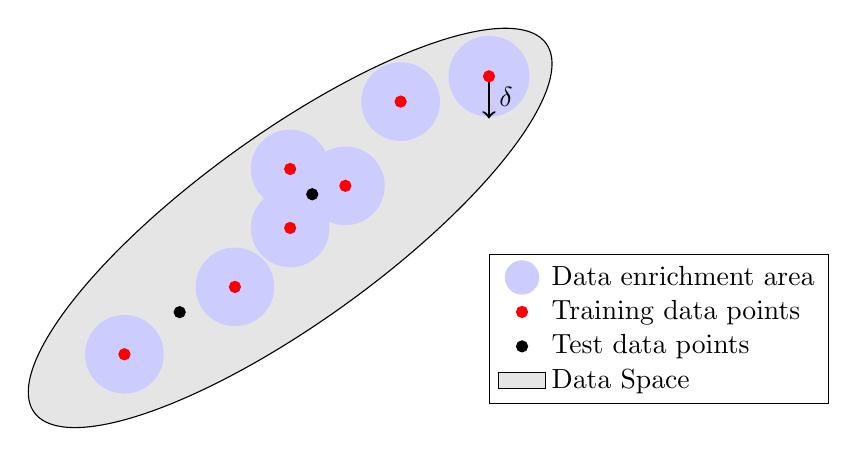
\begin{tikzpicture}
               \begin{axis}[
                xlabel={X-axis label},
                ylabel={Y-axis label},
                width=10cm,
                height=8cm,
                grid=major,
                legend style={at={(.8,.3)},anchor= west, nodes={right}},
                xmin=-3, xmax=3,
                ymin=-3, ymax=3,
                hide axis,
                ]
               \addplot[only marks, mark=*, mark options={scale=7, fill=blue!20, draw=blue!20}, forget plot] coordinates {
                (0,.7)
                (1,1.5)
                (0,0)
                (0.5,0.5)
                (-0.5,-0.7)
                (-1.5,-1.5)
                };
               \addplot[only marks, mark=*, mark options={scale=3, fill=blue!20, draw=blue!20}] coordinates {
                (0,0)
                };
               \addlegendentry{Data enrichment area}
               \addplot[only marks, color=red, mark=*] table [row sep=crcr] {
                x y \\
                0 .7 \\
                1 1.5 \\
                0 0 \\
                .5 .5 \\
                -.5 -.7 \\
                -1.5 -1.5 \\
                1.8 1.8 \\
                };
               \addlegendentry{Training data points}
               \addplot[only marks, color=black, mark=*] table [row sep=crcr] {
                x y \\
                0.2 .4 \\
                -1 -1 \\
                };
               \addlegendentry{Test data points}
               \addplot [
                domain=0:360,
                samples=100,
                smooth,
                variable=\t,
                fill=gray!20,
                forget plot,
                ] (
                {3.2 * cos(\t) * cos(45) - 1 * sin(\t) * sin(45)},
                {3.2 * cos(\t) * sin(45) + 1 * sin(\t) * cos(45)}
                );
               \addlegendimage{area legend, fill=gray!20, draw=black}
               \addlegendentry{Data Space}
               \begin{scope}
               \draw[thick, fill=blue!20, color = blue!20] (axis cs:1.8, 1.8) circle (.5cm);
               \draw[->, thick, black] (axis cs:1.8,1.8) -- (axis cs:1.8,1.3) node[midway, right] {$\delta$};
               \end{scope}
               \end{axis}
               \end{tikzpicture}
        }
        
    \end{column}
    \begin{column}{0.5\textwidth}
        2. Inducing implicit regularization terms, we simultaneously minimize 

        \[\MSE{\Psi{}|_{\ub^{i}} - \mc{F}|_{\ub^{i}}}\] 

        \[  \MSE{\nabla_{\ub}\Psi|_{\ub^{i}} - \nabla_{\ub}\mc{F}|_{\ub^{i}}} \]

        \[  \MSE{\nabla_{\ub}^2\Psi|_{\ub^{i}} - \nabla_{\ub}^2\mc{F}|_{\ub^{i}}} \]

    \end{column}
\end{columns}

}
% \myblue{Improve stability, long-term prediction capacity, and generalization.}

}

